\documentclass[a4paper, 12pt]{exam}

%\usepackage{mathpazo}
\usepackage[onehalfspacing]{setspace}
\usepackage{graphicx}
\usepackage{amsmath, amssymb, amsfonts}
\usepackage[table]{xcolor}
\usepackage{gensymb}
\usepackage[]{booktabs}
\usepackage[utf8]{inputenc}
\usepackage{array}
\usepackage{setspace}
\usepackage{xhfill}
\usepackage{enumitem}
\usepackage{multicol}
\usepackage{mathtools}
%\usepackage{background} %Package for adding a watermark

%\backgroundsetup{scale = 1, angle = 0, firstpage = false, opacity=0.1, contents=\includegraphics{Watermark}}

\newcommand{\dho}{\partial}
\newcommand{\cuspac}{\hspace{0.5cm}}
\newcommand{\longspac}{\hspace{1cm}}
\newcommand{\tripdot}{\cdot \cdot \cdot}


\mathtoolsset{showonlyrefs}

\title{
	{Answers to ADCS Subsystem Test} \\
	\textbf{\large Team Anant Recruitment Test}\\
	\vspace{0.75cm}
	%\includegraphics[scale = 0.5]{Watermark}
}
\date{28th January, 2024}
\author{Pranav Chandra N.V \\ 2023AAPS0013P}


\begin{document}
	\maketitle
	\newpage
	
	{\large\textbf{2. Reaching for the stars.}}
		
		This question is essentially the concept behind a Hohmann transfer orbit\footnote{Thanks to Dev in my SPARKLE project for telling me the name of this process lol}.
		
		We make the following assumptions in order to actually carry out this maneuver:
		\begin{itemize}
			\item Velocity changes to the aircraft occur instantaneously. - The assumption is valid since the burn time of the rocket will likely be much shorter than the period of the orbit\footnote{https://dspace.mit.edu/bitstream/handle/1721.1/60691/16-07-fall-2004/contents/lecture-notes/d30.pdf}.
		\end{itemize}
		
		Using these assumptions, and overall just using the conservation of energy, we can get the following formulae. (Ref. Figure 1)
		
		\begin{figure}[h!]
			\centering
			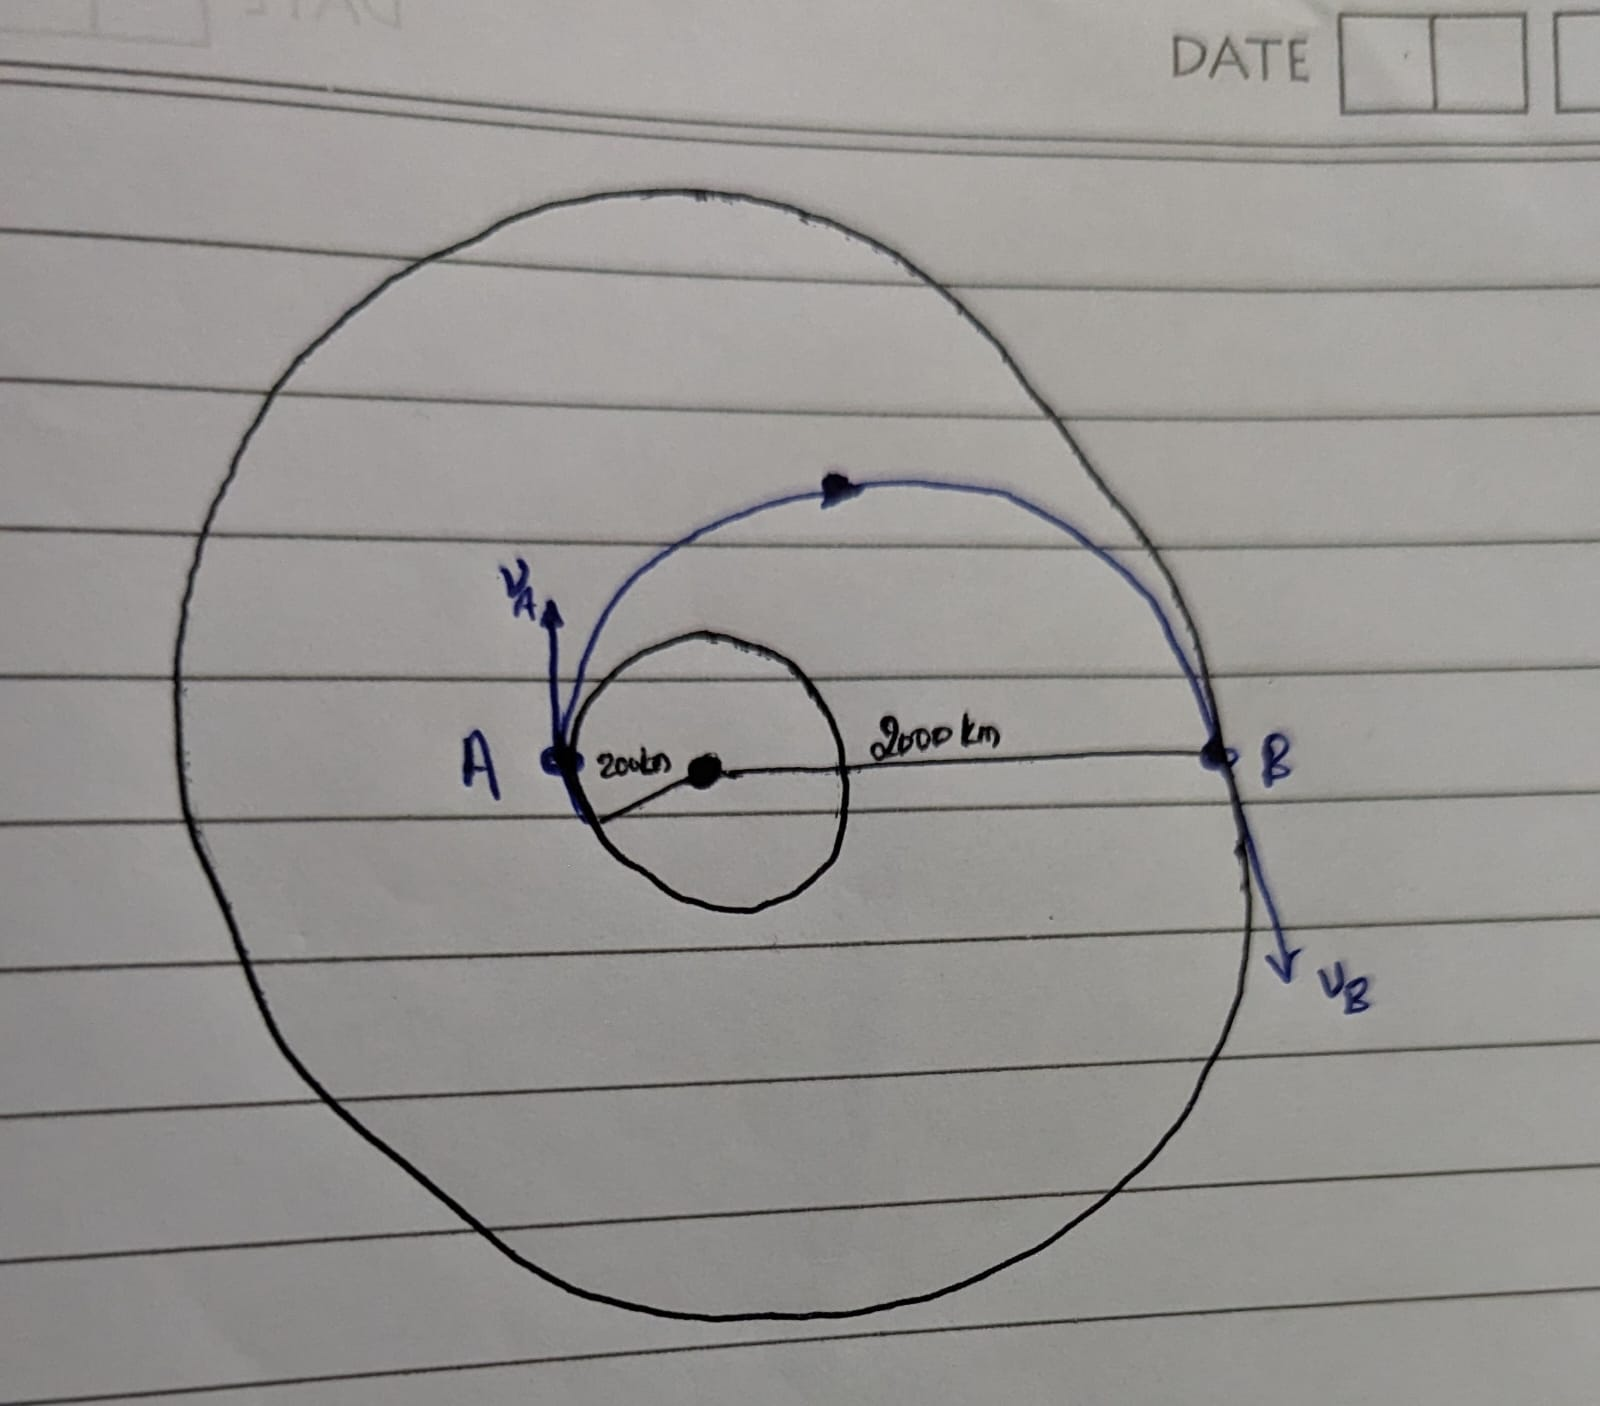
\includegraphics[scale = 0.1]{image1_ADCS}
			\caption{}
		\end{figure}
		Starting from conservation of energy of a small body $m$ in elliptical orbit around a larger body $M$:
		\begin{equation}
			\begin{split}
				T.E = \frac{1}{2}mv^2 - \frac{GMm}{r} = -\frac{GMm}{2a}
			\end{split}
		\end{equation}
		Now solving for $v$:
		\begin{equation}
			v^2 = GM\left(\frac{2}{r} - \frac{1}{a}\right)
		\end{equation}
		Also using the formulas $v_{orbit} = \sqrt{\frac{GM}{r}}$ and $a = \frac{r_1+r_2}{2}$ for orbit at a particular height, we can write the change in velocity at point $A$ as:
		\begin{equation}
			\begin{split}
				\Delta v_A &= \sqrt{GM\left(\frac{2}{r_1} - \frac{2}{r_1 + r_2}\right)} - \sqrt{\frac{GM}{r_1}} \\
				&\Rightarrow \Delta v_1 = \sqrt{\frac{GM}{r_1}}\left(\sqrt{\frac{2r_2}{r_1 + r_2}}-1\right)
			\end{split}
		\end{equation}
		
		Now that we have the equation for $\Delta v_1$, we can plug in our numbers:
		\begin{equation}
			\begin{split}
				r_1 = 200 \times 10^3 + 6.378 \times 10^3 &= 206.378 \times 10^6 m \\
				r_2 = 2000 \times 10^3 + 6.378 \times 10^3 &= 2006.378 \times 10^6 m \\
				M &= 5.972 \times 10^{24} kg
			\end{split}
		\end{equation} 
		Giving us the equation:
		\begin{equation}
			\begin{split}
				\Delta v_1 &= \sqrt{\frac{6.67 \times 10^{-11}\times 5.972 \times 10^{24}}{206.378 \times 10^6}} \left(\sqrt{\frac{2\times2006.378 \times 10^{24} }{(2006.378+206.378)\times10^3}}-1\right)\\
				\Rightarrow \Delta v_1 &= 481.631 m/s
			\end{split}
		\end{equation}
		
		\textbf{Bonus Question:}
		
		To calculate the braking $\Delta v_2$, we use:
		\begin{equation}
			\begin{split}
				\Delta v_2 &= \sqrt{\frac{GM}{r_2}}\left(1-\sqrt{\frac{2r_1}{r_1+r_2}}\right)\\
				\Rightarrow \Delta v_2 &= 789.257 m/s
			\end{split}
		\end{equation}
		
		\newpage
				
		{\large \textbf{4. Lost In The Gaps}}
		\begin{enumerate}
			\item \textbf{Given the first n measurements ${x_1, x_2,\tripdot, x_n}$ estimate the true distance to the car.}
			
			Quite simply, we can use the mean:
			\begin{equation}
				\bar{x} = \frac{\sum_{n = 0}^{n = N}x_n}{N}
			\end{equation}
			However it may be wise to apply a filter and exclude the upper and lower 5\% of all the readings obtained to reduce fluctuations. This will be discussed later.
			
			\item \textbf{It is unfeasible to store data for long periods of time. Rewrite the obtained expression in (1) to use the estimate after $(n-1)^{th}$ measurement (say $x$) and the $n^{th}$ measurement to obtain the new estimate.}
			
			Taking the previous mean to be $\bar{x}_{N-1}$, the current mean to be $\bar{x}_N$ and the incoming measurement to be $x_N$:
			\begin{equation}
				\bar{x}_N = \frac{(\bar{x}_{N-1}\times N)+x_N}{N}
			\end{equation}
			
			\item \textbf{Given the measurements, estimate the distance.}
			
			We will organize the measurements in descending order and apply a filter to remove the top and bottom 5\%, as shown in the image below.
			\begin{figure}[h!]
				\centering
				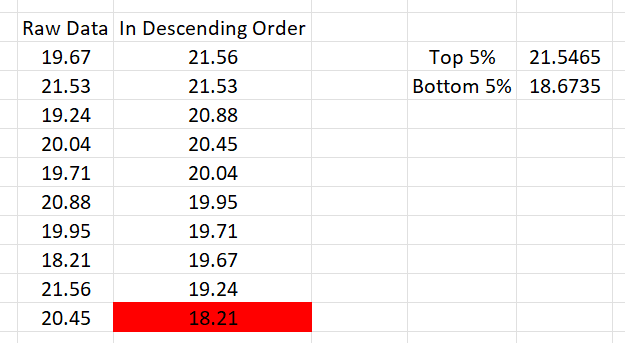
\includegraphics{ADCS_Q4_Image1}
			\end{figure}
			\begin{equation}
				\bar{x}_N = 20.33 m
			\end{equation}
			
			\pagebreak
			
			\item \textbf{Given the first n measurements, estimate the (n + 1)th measurement. (You may use the result obtained in (2)).}
			
			To do this, we will first try to find the initial position and then use $x=vt$ to update subsequent positions.
			
			\begin{equation}
					x_n = x_{n-1} + vt 
			\end{equation}
			\begin{equation}
				\sum_{i = 0}^{i = N}x_i = x_1 + (x_1 + vt) + (x_1 + 2vt) + \tripdot +	(x_1 + (n-1)vt)
			\end{equation}
			\begin{equation}
				\sum_{i = 0}^{i = N}x_i = nx_1 + \frac{(n-1)(n)}{2}vt
			\end{equation}
			\begin{equation}
				x_1 = \frac{\sum_{i = 0}^{i = N}x_i - \frac{(n-1)(n)}{2}vt}{n}
			\end{equation}
			The final part of the above equation gives us a consistently updatable and relaible way to measure the original distance $x_1$, we can now write:
			\begin{equation}
				x_{n+1} = x_1 + nvt
			\end{equation}
		\end{enumerate}
\end{document}